\documentclass[conference]{IEEEtran}

% All these packages you need, if you need any others you can add them here.
\usepackage{graphicx}
\usepackage{amsmath}
\usepackage{booktabs}
\usepackage{hyperref}

% Reduce hyphenation while keeping inter-word spacing tight.
\pretolerance=2000
\hyphenpenalty=800
\exhyphenpenalty=500
\emergencystretch=1em

% Do not change the bibliography style.
\bibliographystyle{IEEEtran}

% ── Project Data ──────────────────────────────────────────────────────────────
\title{Human-Centric Adaptive Assessment: Evaluating Static Rule-Based and Dynamic LLM-Based Mental Health Questionnaires}

\author{
  \IEEEauthorblockN{Jaeyun Ree, Khang Huynh, and Zachary Yeap}
  \IEEEauthorblockA{Department of Software Engineering}
}
% ─────────────────────────────────────────────────────────────────────────────

\begin{document}

\maketitle

% ── Abstract ─────────────────────────────────────────────────────────────────
\begin{abstract}
% TODO: ~150 words
% Hint: Cover (1) problem: static questionnaires fail to reflect changing conditions,
%       (2) approach: Navigator prototype with rule-based and LLM-based methods,
%       (3) study: within-subjects user study, metrics: Clarity / Quality / Relevance,
%       (4) key findings.
Static mental health check-in questionnaires can be clear and clinically
grounded, but they often repeat the same questions regardless of changing
user states. This study presents Navigator, a web-based prototype comparing
a static rule-based monthly check-in with a dynamic LLM-based method that
adapts baseline questions using a controlled persona and previous-month
health profile. Forty valid participants evaluated both methods through a
within-subjects survey grounded in COSMIN content-validity dimensions:
Clarity, Relevance, and Quality. The LLM-based method received higher
composite ratings for Relevance ($d_z=0.58$) and Quality ($d_z=0.59$),
while the Clarity difference was smaller ($d_z=0.41$). Qualitative
responses suggested that participants valued personalisation and
history-aware questioning, while the rule-based method remained
understandable and straightforward. These findings indicate that the main
advantage of LLM-based adaptation lies in contextual relevance rather than
clearer wording alone.
\end{abstract}

% ── Section 1: Introduction ───────────────────────────────────────────────────
\section{Introduction}
\label{sec:intro} 

Mental health is increasingly recognised as a critical component of overall well-being,
and digital health applications are playing a growing role in routine screening and
self-monitoring, such as periodic mood check-ins and longitudinal symptom tracking.
In practice, most of these applications rely on standardised static
instruments such as the PHQ-9 \cite{kroenke2001} and the GAD-7 \cite{spitzer2006},
which present the same fixed set of questions at every check-in regardless of the user's
current condition, prior responses, or longitudinal history. While these instruments
are clinically validated, repeated administration of the same questions can increase
self-report burden and reduce user engagement over time \cite{maatoug2021}.

Adaptive questionnaire techniques, such as pre-determined branching logic and computerised adaptive
screening, have been introduced to partially address this limitation by tailoring question
sequences to user input \cite{wang2023}. However, these static rule-based mechanisms remain
bounded by predefined decision trees and cannot generate non-repetitive new question sets
or dynamically reframe questions based on a user's individual context.
Prior work on computerised adaptive testing has shown that adaptive selection
can reduce question burden while preserving the quality of the measurement
\cite{gibbons2008, choi2010}, further motivating exploration of more flexible
adaptation methods \cite{malanin2025}.

Recent advances in Large Language Models (LLMs) open a new design space for adaptive
assessment: LLMs can synthesise context-aware questions informed by a user's health
profile, lifestyle changes, and prior responses, and have begun to be explored as
engines for patient-reported outcome measures \cite{terheyden2025}. Despite this promise,
the use of LLMs in mental health remains at an early stage. A recent systematic review
of mental health chatbots highlights that most existing systems use pre-determined rule-based questionnaires,
and that LLM-based questionnaire designs, while more flexible, introduce new concerns around safety,
appropriateness, and validation \cite{hua2025, li2025llm, shen2026}.
Despite this growing body of work, to our knowledge, prior studies have not
directly compared LLM-based and rule-based adaptive mental health
questionnaires within a single application using a controlled,
human-centric evaluation grounded in established content-validity criteria
such as relevance, comprehensibility, and comprehensiveness.


To address this gap, we developed \emph{Navigator}, a web-based prototype that
implements two distinct monthly mental health check-in methods within the same
application environment:
\begin{itemize}
  \item \textbf{Static rule-based method:} predefined branching logic determines
        which follow-up questions appear based on fixed risk-level thresholds.
  \item \textbf{Dynamic LLM-based method:} Google Gemini 2.5 Flash adapts
        baseline questions using the user's health profile and prior assessment data.
\end{itemize}
Using a within-subjects study design, participants interacted with both methods via a
standardised persona (Sophie) and completed a structured feedback survey. Evaluation
metrics are grounded in the COSMIN content-validity framework \cite{terwee2018},
which identifies \emph{Clarity}, \emph{Quality}, and \emph{Relevance} as core
dimensions of questionnaire content validity.

This study aims to answer the following research questions:
\begin{itemize}
  \item \textbf{RQ1 (Clarity):} Do LLM-based questionnaires produce higher perceived
        clarity than rule-based questionnaires?
  \item \textbf{RQ2 (Quality):} Do LLM-based questionnaires produce higher perceived
        quality than rule-based questionnaires?
  \item \textbf{RQ3 (Relevance):} Do LLM-based questionnaires produce higher perceived
        relevance than rule-based questionnaires?
\end{itemize}

The main contributions of this work are:
(1) the Navigator prototype, a Flutter web application implementing both rule-based
and LLM-based adaptive questionnaires within a unified interface;
(2) a within-subjects user study design using a standardised persona to ensure fair
comparison across conditions; and
(3) an empirical, COSMIN-grounded evaluation of user perceptions of Clarity, Quality,
and Relevance for LLM-based versus rule-based adaptive mental health questionnaires.

The remainder of this paper is organised as follows.
Section~\ref{sec:related} reviews related work on mental health questionnaire systems,
LLMs in healthcare, and adaptive survey design.
Section~\ref{sec:system} presents the methodology, covering the research
approach, system design, controlled scenario, study design, and
evaluation metrics.
Section~\ref{sec:results} presents the results, followed by discussion in
Section~\ref{sec:discussion}, and conclusions in Section~\ref{sec:conclusion}.

% ── Section 2: Related Work ───────────────────────────────────────────────────
\section{Related Work}
\label{sec:related}

Digital mental health applications increasingly offer routine self-monitoring
through periodic check-ins, yet most rely on static, validated instruments
that repeat the same items regardless of a user's changing condition
\cite{kroenke2001, spitzer2006}. Adaptive approaches, from computerised
adaptive testing to rule-based branching interfaces, have partially addressed
this rigidity, but remain bounded by predefined item banks or decision trees
\cite{gibbons2008, wang2023}. More recently, large language models have been
explored as engines for generating personalised patient-reported outcome items
\cite{terheyden2025}, though their use in mental health is still at an early
stage and raises concerns around safety and validation
\cite{hua2025, shen2026}. Despite this growing body of work, no study has
directly compared rule-based and LLM-based adaptive questionnaires within a
single application using a controlled, human-centric evaluation.

Navigator is a web-based mental health questionnaire prototype developed to
address this gap. It implements both a static rule-based and a dynamic
LLM-based monthly check-in method within the same application environment,
allowing direct comparison under identical conditions. Although the broader
project was initially framed around adaptive assessment across multiple
chronic-disease domains \cite{aihw2012}, this paper narrows the evaluation
to mental health check-ins, which provide a concrete, high-impact, and
survey-feasible context.

We organise prior work along three lines: static mental health
instruments and their limitations; adaptive questionnaire strategies
from CAT to LLM-PROMs; and emerging LLM-based mental health systems with
their associated safety considerations.

\subsection{Mental Health Assessment and Static Instruments}
\label{subsec:rw_static}

Mental health screening in digital health applications has long relied on
standardised fixed-item instruments such as the PHQ-9 \cite{kroenke2001}
and GAD-7 \cite{spitzer2006}, whose brevity and validated scoring make
them attractive for routine longitudinal monitoring. However, the
stability that gives these instruments their psychometric strength also
imposes user-experience limitations: identical items at every
administration can drive fatigue and reduce completion. Ecological
momentary assessment work documents this directly---a 28-day
smartphone-based depression study reported a 62.5\% average daily
response rate with only seven of eleven participants completing the full
protocol \cite{maatoug2021}---and recent work has explicitly called for
more adaptive health questionnaires \cite{malanin2025}.

Fixed wording also raises content-validity concerns. Baas et~al.\
\cite{baas2011} found measurement non-invariance for a PHQ-9 item across
ethnic groups, and Wild et~al.\ \cite{wild2005} argue that questionnaire
wording must be treated as a structured design and validation problem.
Even well-validated instruments thus carry implicit assumptions about the
respondent that adaptive systems may help mitigate through
context-sensitive wording and item selection.

\subsection{Adaptive Questionnaire Approaches}
\label{subsec:rw_adaptive}

To mitigate the rigidity of static instruments, prior work has explored
adaptive questioning. Computerised Adaptive Testing (CAT) uses item
response theory to select the most informative items from a validated
bank: Gibbons et~al.\ \cite{gibbons2008} reduced administered items by
$\sim$95\% while preserving full-scale correlation, and Choi et~al.\
\cite{choi2010} showed that CAT outperforms static short forms on most
PROMIS depression criteria. In broader health contexts, Wang et~al.\
\cite{wang2023} identify rule-based ``if--then'' logic as the dominant
adaptation paradigm for chronic-disease interfaces, valued for
interpretability but bounded by the designer's predefined rules.

A more recent direction extends adaptation from item \emph{selection} to
item \emph{generation}. Terheyden et~al.\ \cite{terheyden2025} introduce
LLM-powered Patient-Reported Outcome Measures (LLM-PROMs), in which large
language models generate personalised items grounded in validated
psychometric content. This conceptual shift defines the design space we
examine: unlike CAT, LLM-based methods can also rewrite wording and
generate follow-up prompts, creating both personalisation opportunities
and new validity risks.

\subsection{LLM-Based Systems in Mental Health}
\label{subsec:rw_llm_mh}

LLMs have accelerated interest in conversational mental health tools,
but evidence on their efficacy and safety remains preliminary. Hua et~al.\
\cite{hua2025} surveyed 160 mental health chatbot studies (2020--2024)
and found that LLM-based systems, though rapidly growing, remain
concentrated in early-stage validation while rule-based systems still
dominate later-stage human and clinical testing---positioning our work
as a user-centred feasibility evaluation rather than a clinical efficacy
trial. User-facing evidence further suggests LLM behaviour is
condition-dependent: Li et~al.\ \cite{li2025llm} report
condition-specific differences in user sentiment, and Shen et~al.\
\cite{shen2026} found that no tested model reliably produced appropriate
responses to psychotic content. These findings establish two requirements
for LLM-based mental health tools: condition-aware framing and explicit
safety boundaries. Importantly, questionnaire systems differ from
therapeutic dialogue---they elicit structured self-reports through clear
prompts---so conversational LLM risks translate, but do not transfer
directly, into questionnaire design constraints.

Despite this growing body of work, no prior study has directly compared
rule-based and LLM-based adaptive questionnaires within a unified
application using a controlled, within-subjects evaluation. Existing
comparisons either contrast chatbot generations \cite{hua2025}, study
unstructured LLM use \cite{li2025llm}, or evaluate item \emph{selection}
without addressing LLM-based \emph{wording} \cite{gibbons2008,
choi2010}. Our work addresses this gap by holding the application,
persona, and participant group constant, isolating the adaptation method
itself.

Although several evaluation approaches exist for patient-reported outcome
measures, the COSMIN (COnsensus-based Standards for the selection of health
Measurement INstruments) framework \cite{terwee2018} is widely recognised as
the methodological standard for assessing content validity. Drawing on an
international Delphi study of 159 experts, COSMIN formalises content validity
along three dimensions: \emph{relevance}, \emph{comprehensiveness}, and
\emph{comprehensibility}. These dimensions align directly with the evaluation
needs of this study, as described in Section~\ref{subsec:metrics}.

In summary, existing work shows that adaptive item selection reduces
respondent burden, LLM-based mental health tools are growing but remain
at early validation stages, and COSMIN provides the established framework
for evaluating content validity. No prior study, however, has directly
compared static rule-based and dynamic LLM-based adaptive questionnaires
within a single application using a controlled, human-centred,
COSMIN-grounded evaluation---the gap this study addresses.

% ── Section 3: Methodology ───────────────────────────────────────────────────
\section{Methodology}
\label{sec:system}

The methodology comprises four components: (i)~implementation of two
adaptation methods within a unified web-based prototype
(Sections~\ref{subsec:architecture}--\ref{subsec:llm_based}); (ii)~a
controlled evaluation scenario built around a standardised persona
(Section~\ref{subsec:sophie}); (iii)~a within-subjects user study with a
COSMIN-grounded feedback survey
(Sections~\ref{subsec:research_design}--\ref{subsec:metrics}); and
(iv)~data collection and analysis (Section~\ref{subsec:data_collection}).
The prototype is designed as an evaluation instrument rather than a
production system, so architectural choices---shared interface, fixed
persona, identical health domains---are driven by the comparison design.

\subsection{Architecture Overview}
\label{subsec:architecture}

Navigator is implemented as a Flutter web application backed by
Supabase (PostgreSQL) for question storage and branching-rule
definitions. The single-page interface presents foundational intake
questions, monthly check-ins, and a results dashboard. The broader
prototype supports six health domains, but this study evaluates only
the Mental Health pathway. Both methods share the same front-end
layout, rendering components, and scoring pipeline, so any observed
difference is attributable to the adaptation method rather than
interface variation. The prototype presents a pre-filled foundational
assessment (Step~1) followed by the two monthly check-in pathways
(Step~2); Figure~\ref{fig:persona_reference} shows the persona
reference provided to participants beforehand.

\begin{figure}[t]
  \centering
  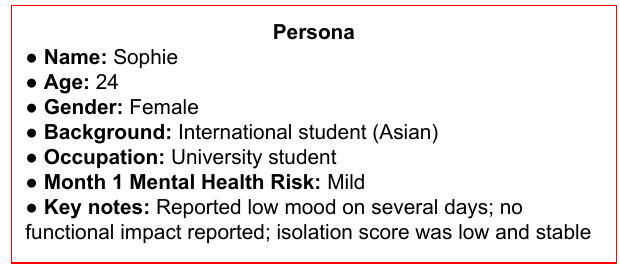
\includegraphics[width=0.82\columnwidth]{figures/persona_reference.png}
  \caption{Persona reference shown to participants in the user guide, defining Sophie's demographic profile, Month~1 mental health risk level, and key context notes used as the Month~0/Month~1 input for the adaptive check-in.}
  \label{fig:persona_reference}
\end{figure}

For LLM-based generation, the application calls the Google Gemini~2.5
Flash API. Before final implementation, the team conducted an informal
feasibility check of three candidate LLM providers---Gemini, an OpenAI
GPT model, and an Anthropic Claude model---using the Sophie scenario
and the same structured-output requirement. This check was not a formal
model benchmark and was not used to make general claims about model
quality; it was used only to select an implementable provider for the
prototype. Gemini~2.5 Flash was selected because its pilot outputs
preserved the intended mental health constructs, produced usable
personalised wording, and followed the required JSON schema. The
selection was also supported by practical considerations aligned with
the prototype: a free-tier API quota that supports reproducibility,
native JSON response mode that maps directly to the questionnaire
schema, low inference latency suitable for real-time web use, and Google
Cloud integration alongside the Flutter and Supabase stack. We acknowledge
that reliance on a single LLM provider limits generalisability (see
Section~\ref{subsec:limitations}). A deterministic fallback path
returns pre-authored enhanced questions if the API is unavailable,
ensuring identical content across participants.

\subsection{Static Rule-Based Adaptation Method}
\label{subsec:rule_based}

The rule-based method adapts the monthly check-in through a branching
engine that evaluates predefined \emph{trigger--condition--action}
rules: when a user answers a trigger question, the engine evaluates the
condition against the response and shows or hides target questions
accordingly---the ``if--then'' paradigm identified as dominant in
chronic-disease adaptive interfaces \cite{wang2023}. Critically, each
rule operates on single-question, single-timepoint data and cannot
access prior-month responses or aggregate longitudinal patterns. For
the Mental Health domain, risk levels are classified using
percentage-based thresholds loosely inspired by the PHQ-9 severity bands
\cite{kroenke2001}: $<$25\% \emph{None}, 25--50\% \emph{Mild}, 50--75\%
\emph{Moderate}, $>$75\% \emph{High}. These thresholds are a simplified
prototype mapping and do not correspond to PHQ-9 cut-off scores
(5, 10, 15, 20). Sophie's scenario in Table~\ref{tab:comparison}
illustrates the resulting limitation: Rule~13 hides the
functional-impact item when the mood-frequency response is $<2$, so her
Month~2 response of~1 (``Several days'') suppresses the item despite a
clinically meaningful two-month Mild pattern that the rule cannot detect.

\subsection{Dynamic LLM-Based Adaptation Method}
\label{subsec:llm_based}

The LLM-based method conditions a large language model on the user's
prior health snapshot. At the start of each check-in, the system
constructs a structured prompt with two inputs: (i)~a \emph{UserSeed}, a
versioned summary of the user's demographics, domain-level risk
classifications, and free-text context notes from the previous
assessment period; and (ii)~the baseline rule-based questions for the
current domain, so the model knows what it is improving upon. The
prompt instructs the model to produce questions that are \emph{more
relevant, clearer, and less repetitive} than the baseline, grounding the
task in the same Clarity/Quality/Relevance dimensions used in evaluation
(Section~\ref{subsec:metrics}). The model returns a JSON array of
question objects (text, response options, adaptation rationale) at a
low temperature setting ($T=0.3$) to favour consistency over creative
variation. A simplified excerpt of the prompt:

\begin{quote}
\small
\textit{You are a compassionate health questionnaire assistant. Given the
user's previous assessment summary below, adapt the baseline check-in
questions to be more relevant, clearer, and less repetitive.}

\textit{UserSeed: \{name: Sophie, age: 24, occupation: university student,
domain: Mental Health, month1\_risk: Mild, context: ``Reported difficulty
sleeping and managing coursework stress''\}}

\textit{Baseline questions: [list of 5 rule-based items for Mental Health
domain]}

\textit{Return a JSON array where each object contains: question\_text,
response\_options, and adaptation\_rationale. Do not introduce new clinical
domains; rephrase, re-prioritise, or add follow-up items only when supported by
the user's longitudinal context.}
\end{quote}

This design aligns with the LLM-PROM framework \cite{terheyden2025},
which argues that LLM-generated patient-reported outcome items should be
developed from validated content and benchmarked against fixed
instruments. In Navigator the LLM does not generate from scratch but
\emph{transforms} baseline items using the user's longitudinal context.
Table~\ref{tab:comparison} summarises the resulting transformations in
Sophie's scenario, mapped to COSMIN dimensions.

\begin{table*}[t]
\caption{Mental health check-in questions under each adaptation method for Sophie's Month~2 scenario, mapped to COSMIN content-validity dimensions. The rule-based column shows the questions produced by the branching engine; the LLM-based column shows the Gemini~2.5 Flash-assisted transformations.}
\label{tab:comparison}
\centering
\small
\begin{tabular}{@{}p{1.8cm}p{1.5cm}p{3.6cm}p{4.0cm}p{4.8cm}@{}}
\toprule
\textbf{Item} & \textbf{COSMIN} & \textbf{Rule-Based} & \textbf{LLM-Based} & \textbf{Transformation Rationale} \\
\midrule
Mood frequency
& Clarity
& ``In the past month, how often have you felt low mood, sad, hopeless, nervous, worried, or restless?''
& ``Over the past month, have you continued to experience feelings like low mood, worry, or restlessness? Last month you reported this happening on several days.''
& References Month~1 history; acknowledges continuity rather than repeating identical wording. \\
\addlinespace
Managing life
& Clarity
& ``\ldots how often have you felt that important things in your life were difficult to manage?''
& ``\ldots has it felt harder than usual to stay on top of your studies, daily responsibilities, or relationships?''
& Replaces generic ``important things'' with student-specific language. \\
\addlinespace
Trend direction
& Relevance
& Not asked
& ``Since you've reported similar feelings for two months in a row, how would you describe the change over the past month?''
& New item capturing longitudinal signal (two-month Mild pattern) that rule-based thresholds cannot detect. \\
\addlinespace
Functional impact
& Quality
& \emph{Hidden} because the mood score of~1 does not meet the $\geq 2$ threshold required by the branching rule.
& ``Have these feelings made it harder for you to manage your daily life, for example, attending classes, completing work, or maintaining relationships?''
& Unlocked early based on persistent pattern; phrasing adapted to student context. \\
\addlinespace
Assessment coverage
& Quality
& Visible questions focus mainly on current symptom frequency and generic manageability; functional consequence is absent when the threshold is not met.
& Visible questions cover symptom continuity, student responsibilities, change direction, and functional impact.
& Improves completeness of the monthly assessment by collecting both symptom status and practical impact. \\
\addlinespace
Isolation
& Relevance
& ``In the past month, how often do you feel isolated from others?''
& \emph{Skipped} because the Month~1 score was low and stable, so no new information was expected.
& De-prioritises items unlikely to yield new signal, reducing respondent burden. \\
\bottomrule
\end{tabular}
\end{table*}

\begin{figure*}[t]
  \centering
  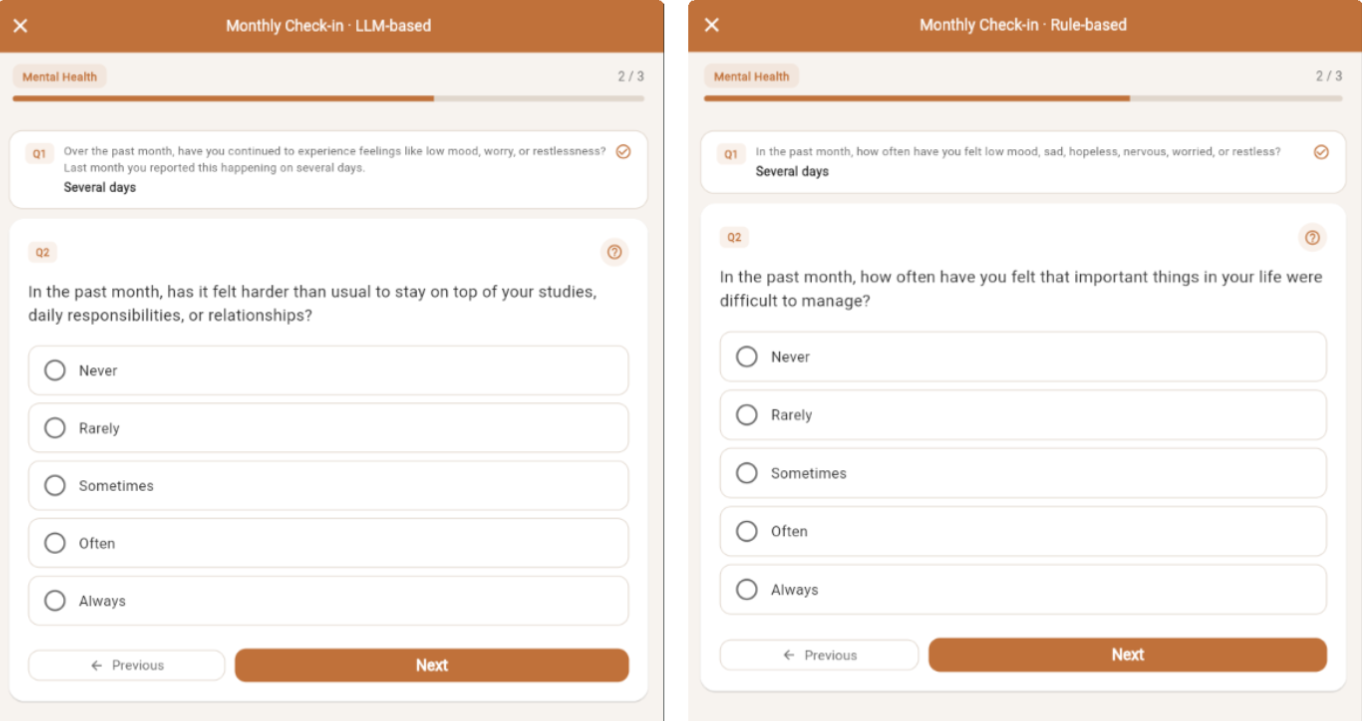
\includegraphics[width=0.75\textwidth]{figures/static_llm_comparison.png}
  \caption{Side-by-side comparison of Sophie's Month~2 mental health check-in. Left: the LLM-based method adapts question wording using Sophie's prior history and student context. Right: the rule-based method presents the same generic questions regardless of the user's profile.}
  \label{fig:method_comparison}
\end{figure*}

\subsection{Controlled Scenario: Sophie}
\label{subsec:sophie}

To enable a fair within-subjects comparison, both methods are evaluated
using a single standardised persona---a predetermined profile presented
identically to every participant---rather than participants' own health
data. ``Sophie'' is a fictional 24-year-old female East Asian
international university student whose Month~1 assessment produced a
\emph{Mild} mental health risk and \emph{None} across other domains
(see Figure~\ref{fig:persona_reference}). Her context records a
mood-frequency score of~1 (``Several days''), a low and stable isolation
score, and no triggered functional-impact questions.

The fixed persona serves three purposes. First, it eliminates
between-participant variation in health profiles, so observed
differences reflect the adaptation method rather than individual
circumstances. Second, it avoids the ethical complications of
collecting real mental health data in a prototype evaluation. Third, it
concretely illustrates the rule-based limitation: Sophie's profile is
constructed so the branching rule's hard threshold blocks the
functional-impact question despite a clinically meaningful two-month
pattern (Table~\ref{tab:comparison}). The persona also reflects
measurement-validity considerations from prior work---PHQ-9 responses
can exhibit non-invariance across demographic groups \cite{baas2011}
and questionnaire wording must account for cultural context
\cite{wild2005}---so the East Asian international student profile
represents a demographic for whom culturally adapted wording (e.g.,
coursework stress, adjusting to a new country) is particularly relevant.
This design intentionally prioritises internal validity and standardised
comparison over ecological realism.

% ── Study Design (subsections within Methodology) ────────────────────────────
\subsection{Study Design}
\label{subsec:research_design}
\label{sec:study}

The study uses a within-subjects design: every participant interacts
with both methods and rates each on identical evaluation items, with
each participant serving as their own control. A fixed presentation
order (rule-based first, LLM-based second) was adopted because the
rule-based condition establishes a baseline against which LLM
adaptations become interpretable. Counterbalancing was not implemented;
we acknowledge this as a limitation discussed in
Section~\ref{subsec:limitations}. The study was approved by the Monash
University Human Research Ethics Committee (MUHREC; Project ID~51664,
Non-HREC Lower Risk review). All participants provided written informed
consent.

\subsection{Participants}
\label{subsec:participants}

Participants were recruited through convenience sampling via peers,
classmates, and personal networks. Eligibility required adults aged
18+, including university students and working professionals; no
compensation was offered. Per the ethics approval (scoped to the
Australian campus), students at the Monash Malaysia and Indonesia
campuses were excluded. Of 42 responses received between 25~April and
13~May~2026, one non-consent and one invalid submission were excluded,
yielding $n=40$ valid responses (demographics in
Section~\ref{subsec:demographics}).

\subsection{Procedure}
\label{subsec:procedure}

Each participant completed the study independently in a single 10--15
minute session: (1)~\textbf{Orientation}---a user guide introduced the
prototype and the Sophie persona, instructing participants to evaluate
from Sophie's perspective; (2)~\textbf{Rule-based check-in}---Sophie's
Month~2 mental health check-in via the branching engine, in which the
functional-impact item remained hidden because the threshold was not
met (Table~\ref{tab:comparison}); (3)~\textbf{LLM-based check-in}---the
same Month~2 check-in via the LLM method, with identical interface
layout; and (4)~\textbf{Feedback survey} on an external Google Form
with five sections: A~(Demographics), B~(Clarity), C~(Relevance),
D~(Quality), and E~(Overall Experience). Sections~B--D each contained
three 5-point Likert items rated side-by-side for both methods (nine
paired items in total); Section~E asked participants to endorse
satisfaction options (rule-based, LLM-based, both, or neither) and
provide free-text feedback. Sections~B, D, and~E each included one
open-ended prompt (three in total).

\subsection{Evaluation Metrics}
\label{subsec:metrics}

We adopt the COSMIN content-validity framework \cite{terwee2018}
because it is the most widely adopted standard for evaluating the
content validity of patient-reported outcome measures, grounded in an
international Delphi consensus of 159 experts. This provides a
principled comparison basis drawn from established methodology rather
than ad-hoc usability heuristics. The three COSMIN dimensions map onto
study-specific metrics as follows:

\begin{itemize}
  \item \textbf{Clarity} (COSMIN \emph{comprehensibility}): whether
        wording is clear and easy to understand.
  \item \textbf{Quality} (COSMIN \emph{comprehensiveness}): a
        study-specific operationalisation of perceived
        comprehensiveness and assessment usefulness, capturing whether
        questions are well-formed, meaningful, and complete within the
        monthly check-in context.
  \item \textbf{Relevance} (COSMIN \emph{relevance}): whether questions
        are pertinent to Sophie's health profile and circumstances.
\end{itemize}

Each dimension was measured using three 5-point Likert items
(1~\emph{Strongly Disagree} to~5~\emph{Strongly Agree}), presented as
side-by-side matrices in which participants rated both methods on the
same screen (nine paired items, 18~data points per participant). Items
within a dimension were averaged into a composite score per method. The
three open-ended prompts described above complement the Likert data by
surfacing themes that structured items may not capture.

\subsection{Data Collection and Analysis}
\label{subsec:data_collection}

Survey responses were collected via Google Forms between 25~April and
13~May~2026, yielding 42 submissions. Two responses were excluded during
data cleaning: one participant did not provide consent, and one submission
was identified as invalid based on uniform extreme ratings across all
18~Likert items combined with non-substantive open-ended answers.
The final analysis sample comprised $n = 40$ valid responses.

For quantitative analysis, paired-sample $t$-tests were used to compare
composite scores between the two methods for each COSMIN dimension. Effect
sizes were computed using Cohen's $d_z = t / \sqrt{n}$ to characterise the
practical magnitude of observed differences. Item-level tests are reported
descriptively; interpretation focuses on the three pre-specified composite
dimensions. Internal consistency was acceptable across the method-specific
three-item composites (Cronbach's $\alpha=.74$--$.87$). As a robustness
check for the ordinal Likert data, Wilcoxon signed-rank tests were also
computed for the three composite differences. For qualitative analysis,
one researcher coded all open-ended responses inductively, and a second
researcher reviewed the resulting code map for consistency before recurring
themes were grouped thematically.

% ── Section 5: Results and Analysis ──────────────────────────────────────────
\section{Results and Analysis}
\label{sec:results}

\subsection{Participant Demographics}
\label{subsec:demographics}

Table~\ref{tab:demographics} summarises the sample characteristics
($n=40$).
The majority of participants were aged 21--25 (65.0\%) and enrolled as
university students (70.0\%). Gender was approximately balanced, with
21~female (52.5\%) and 19~male (47.5\%) respondents. Most participants
reported low familiarity with health applications: 75.0\% selected
responses indicating rare or no use of such tools. This low adoption
rate reinforces the need to develop accessible and engaging health
check-in tools for university students of all genders, as both female
and male respondents were similarly unfamiliar with existing solutions.

\begin{table}[t]
\caption{Participant demographics ($n = 40$).}
\label{tab:demographics}
\centering
\small
\begin{tabular}{@{}llrc@{}}
\toprule
\textbf{Variable} & \textbf{Category} & \textbf{n} & \textbf{\%} \\
\midrule
Age range   & 18--20  &  8 & 20.0 \\
            & 21--25  & 26 & 65.0 \\
            & 26--34  &  6 & 15.0 \\
\addlinespace
Gender      & Female  & 21 & 52.5 \\
            & Male    & 19 & 47.5 \\
\addlinespace
Role        & Student & 28 & 70.0 \\
            & Working professional & 12 & 30.0 \\
\bottomrule
\end{tabular}
\end{table}

\subsection{Quantitative Comparison}
\label{subsec:quant}

Each of the three COSMIN-grounded dimensions was measured by three
Likert items (1--5 scale). Per-participant composite scores were
computed by averaging the three items within each dimension.
Table~\ref{tab:quant} presents per-item and composite means for both
methods, together with paired $t$-test results ($df = 39$).

All three composite scores were significantly higher for the LLM-based
method: Clarity ($\Delta = +0.13$, $p = .014$), Relevance
($\Delta = +0.42$, $p < .001$), and Quality ($\Delta = +0.29$,
$p < .001$). Relevance showed the largest difference, while Clarity
showed the smallest. Wilcoxon signed-rank sensitivity checks supported
the same direction of effects, with strongest evidence for Relevance and Quality (Clarity $p=.018$; Relevance $p<.001$; Quality $p<.001$).


\begin{table*}[t]
\caption{Per-item and composite Likert scores (mean $\pm$ SD) with paired $t$-test results ($n = 40$). Effect size $d_z = t/\sqrt{n}$. Asterisks: {*}\,$p < .05$; {**}\,$p < .01$; {***}\,$p < .001$.}
\label{tab:quant}
\centering
\small
\begin{tabular}{@{}llcccccc@{}}
\toprule
\textbf{Dimension} & \textbf{Item} & \textbf{LLM (M $\pm$ SD)} & \textbf{Rule (M $\pm$ SD)} & \textbf{$\Delta$} & \textbf{$t$} & \textbf{$p$} & \textbf{$d_z$} \\
\midrule
Clarity
  & Clear and easy to understand      & $4.22 \pm 0.73$ & $4.03 \pm 0.95$ & $+0.20$ & $1.75$ & $.088$ & $0.28$ \\
  & Specific and unambiguous           & $3.83 \pm 0.96$ & $3.70 \pm 1.07$ & $+0.12$ & $1.30$ & $.200$ & $0.21$ \\
  & Easy to know how to answer         & $4.10 \pm 0.96$ & $4.03 \pm 1.05$ & $+0.07$ & $0.62$ & $.538$ & $0.10$ \\
  & \textbf{Composite}                 & $\mathbf{4.05 \pm 0.73}$ & $\mathbf{3.92 \pm 0.84}$ & $\mathbf{+0.13}$ & $\mathbf{2.58}$ & $\mathbf{.014}$* & $\mathbf{0.41}$ \\
\addlinespace
Relevance
  & Relevant to Sophie's health profile & $4.15 \pm 0.66$ & $3.77 \pm 0.80$ & $+0.38$ & $3.55$ & $.001$** & $0.56$ \\
  & Addressed important aspects         & $4.00 \pm 0.75$ & $3.62 \pm 0.87$ & $+0.38$ & $2.94$ & $.005$** & $0.46$ \\
  & Reflected changes since prev.\ month & $4.10 \pm 0.78$ & $3.60 \pm 0.93$ & $+0.50$ & $3.29$ & $.002$** & $0.52$ \\
  & \textbf{Composite}                  & $\mathbf{4.08 \pm 0.63}$ & $\mathbf{3.67 \pm 0.77}$ & $\mathbf{+0.42}$ & $\mathbf{3.69}$ & $\mathbf{<.001}$*** & $\mathbf{0.58}$ \\
\addlinespace
Quality
  & Captured important details           & $3.90 \pm 0.74$ & $3.50 \pm 0.88$ & $+0.40$ & $3.57$ & $.001$** & $0.56$ \\
  & Well designed for meaningful assessment & $4.00 \pm 0.78$ & $3.58 \pm 0.93$ & $+0.42$ & $3.60$ & $.001$** & $0.57$ \\
  & Natural and appropriate              & $3.98 \pm 0.89$ & $3.92 \pm 0.80$ & $+0.05$ & $0.36$ & $.720$ & $0.06$ \\
  & \textbf{Composite}                  & $\mathbf{3.96 \pm 0.65}$ & $\mathbf{3.67 \pm 0.73}$ & $\mathbf{+0.29}$ & $\mathbf{3.76}$ & $\mathbf{<.001}$*** & $\mathbf{0.59}$ \\
\bottomrule
\end{tabular}
\end{table*}

\subsection{Clarity}
\label{subsec:clarity_results}
% TODO: Report per-item and composite Clarity scores.
%       LLM mean 4.08 vs Rule 3.94 -- smallest gap of the three dimensions.
%       Both methods rated positively; suggests both were clearly worded.
%       Interpret: wording clarity is less sensitive to static vs dynamic distinction.

Both methods were rated positively for Clarity, with all item means above~3.7.
The LLM-based method scored slightly higher on each item: clear and easy to
understand ($M=4.22$ vs.~$4.03$), easy to know how to answer ($M=4.10$
vs.~$4.03$), and specific and unambiguous wording ($M=3.83$ vs.~$3.70$).
However, these item-level differences were small, ranging from $+0.07$ to
$+0.20$. The composite Clarity score was significantly higher for the
LLM-based method ($t(39)=2.58$, $p=.014$), but the small difference indicates
that both versions were generally understandable. Descriptively,
wording specificity was the lowest-rated clarity item for both methods,
suggesting a shared design challenge rather than an issue unique to
either approach.

Open-ended responses supported this interpretation. Most respondents who
answered the clarity question reported no confusion, with only isolated
comments mentioning timeframe ambiguity, a need for clearer onboarding, or
LLM-based questions feeling longer. This suggests that the rule-based method
was not unclear; instead, the LLM-based method offered a modest clarity
advantage while preserving overall comprehensibility. This modest
difference is expected: clarity depends primarily on careful question
writing, which was present in both methods, whereas the LLM's
context-aware rephrasing (e.g., referencing Sophie's occupation or
recent mood trend) may have made individual items feel slightly more
concrete and therefore easier to interpret.

\subsection{Relevance}
\label{subsec:relevance_results}
% TODO: Report per-item and composite Relevance scores.
%       LLM mean 4.09 vs Rule 3.68 -- LARGEST gap (+0.40).
%       Key item: "Reflected changes since previous month" shows biggest LLM advantage.
%       Interpret: context-awareness and longitudinal history drive relevance perception.
%       This is the dimension where static vs dynamic distinction is most visible.

Relevance showed the clearest separation between methods. The LLM-based method
was rated higher on all three relevance items: relevance to Sophie's health
profile ($M=4.15$ vs.~$3.77$), addressing what seemed most important
($M=4.00$ vs.~$3.62$), and reflecting changes since the previous month
($M=4.10$ vs.~$3.60$). The largest item-level gap was therefore the
change-tracking item ($\Delta=+0.50$), which directly reflects the LLM method's
ability to use Sophie's longitudinal context.

The composite Relevance score also showed the largest overall difference among
the three dimensions ($\Delta=+0.42$, $t(39)=3.69$, $p<.001$). This result
aligns with the intended distinction between the two approaches. The
rule-based method could ask clear predefined questions, but it could not
automatically connect Sophie's Month~2 questions with her Month~1 profile
unless those pathways were manually encoded. The LLM-based method was
therefore perceived as more relevant because it could adapt question wording
and selection to the persona's previous state.

\subsection{Quality}
\label{subsec:quality_results}
% TODO: Report per-item and composite Quality scores.
%       LLM mean 3.96 vs Rule 3.68 -- moderate gap (+0.27).
%       Interpret: LLM questions felt more meaningful and well-designed overall.

Quality ratings also favoured the LLM-based method, though the pattern was more
specific than a general improvement in user experience. The LLM-based method
scored higher for capturing important details ($M=3.90$ vs.~$3.50$) and being
well designed for a meaningful assessment ($M=4.00$ vs.~$3.58$). In contrast,
the natural and appropriate item was almost tied ($M=3.98$ vs.~$3.92$),
showing that participants did not necessarily experience the LLM version as
more comfortable or natural to complete.

The composite Quality score was significantly higher for the LLM-based method
($\Delta=+0.29$, $t(39)=3.76$, $p<.001$). This suggests that participants
viewed the LLM-based transformations as better aimed at Sophie's situation,
particularly in terms of capturing meaningful details, rather than simply as a
more pleasant interaction.

\begin{figure*}[t]
  \centering
  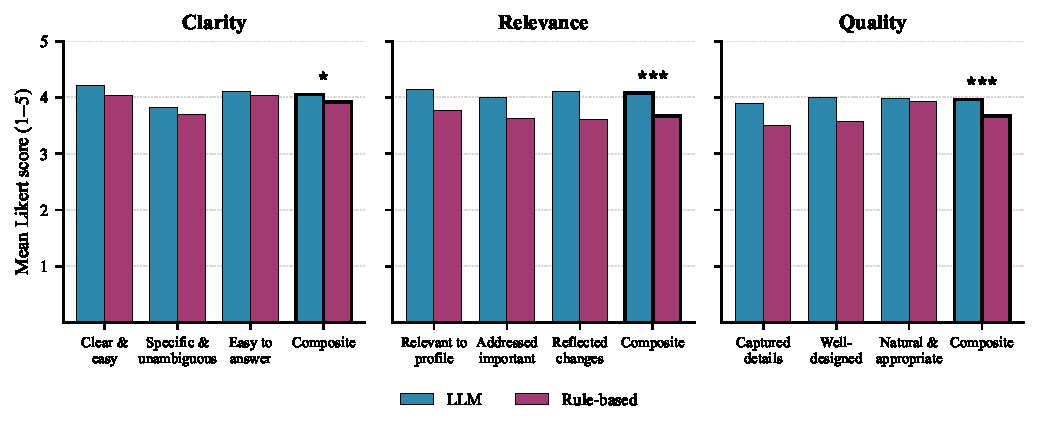
\includegraphics[width=0.88\textwidth]{figures/cosmin_combined.pdf}
  \caption{Per-item and composite Likert ratings across the three COSMIN dimensions for both methods ($n=40$). Composite bars are outlined more boldly; significance markers above each composite denote paired $t$-test results ({*}\,$p<.05$; {***}\,$p<.001$). Clarity differences were small; Relevance and Quality showed larger LLM advantages, with the change-tracking Relevance item exhibiting the single largest item-level gap ($\Delta=+0.50$).}
  \label{fig:cosmin_combined}
\end{figure*}

\subsection{Overall Preference}
\label{subsec:preference_results}
% TODO: Report preference distribution (n=39):
%       Satisfied with both:    17 (43.6%)
%       Dynamic LLM-based:      12 (30.8%)
%       Static Rule-based:       8 (20.5%)
%       Neither:                  2 (5.1%)
%       Interpretation: largest group preferred both -- rule-based was not poor.
%       Combined LLM preference (LLM only + both) = 74.4%.

The overall satisfaction item was multi-select, so responses indicate
endorsement rather than mutually exclusive preference. A majority of
participants endorsed satisfaction with both methods ($n=22$, 55.0\%). The
LLM-based method was endorsed by 17 participants (42.5\%), while the
rule-based method was endorsed by eight participants (20.0\%). Two
participants (5.0\%) selected neither.

These results show broad acceptance of both methods, but stronger endorsement
for the LLM-based version. The large ``satisfied with both'' group indicates
that the rule-based method was not perceived as poor; rather, the LLM-based
method appeared to add personalisation and awareness of prior history.
Figure~\ref{fig:satisfaction} illustrates the distribution.

\begin{figure}[t]
  \centering
  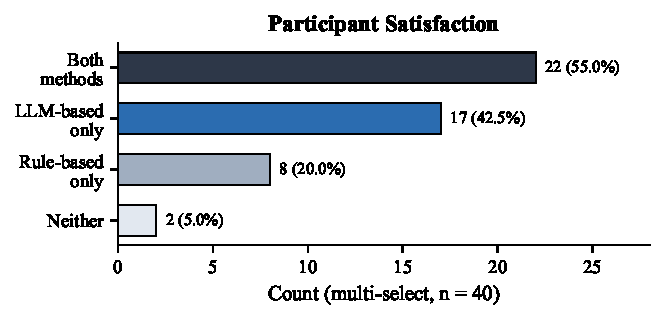
\includegraphics[width=0.9\columnwidth]{figures/satisfaction.pdf}
  \caption{Participant satisfaction endorsements (multi-select, $n=40$). A majority endorsed both methods, with stronger endorsement for the LLM-based version.}
  \label{fig:satisfaction}
\end{figure}

\subsection{Qualitative Findings}
\label{subsec:qual}
% TODO: Thematic analysis of open-ended responses (theme → code → % → quote).
%       Q2 themes (n=39):
%         Personalisation/Relevance       8 (20.5%) -- "The LLM felt more specific and tailored" (P23)
%         No strong preference / Both OK 11 (28.2%) -- "Both were easy to complete" (P33)
%         Longitudinal awareness          4 (10.3%) -- "LLM linked back to Month 1 questions" (P16)
%         Simplicity/Transparency (Rule)  4 (10.3%) -- "Rule-based gave more context of prev. month" (P38)
%         Natural/Conversational          3  (7.7%) -- "LLM feels more human-like" (P05)
%       Q3 improvement themes:
%         More personalisation in LLM     3  (7.7%)
%         Better guidance/instructions    2  (5.1%)
%         User control/flexibility        1  (2.6%)

The open-ended responses helped explain why the LLM-based method was rated
more favourably, particularly in Relevance. Responses were analysed using
an inductive thematic coding approach: one researcher read all responses,
assigned initial codes to meaningful segments, and then grouped related
codes into higher-level themes. A second researcher reviewed the resulting
code map to verify consistency. Table~\ref{tab:qual_preference}
summarises non-mutually-exclusive thematic codes from the comparison question
($n=39$ non-blank responses). Twenty respondents explicitly preferred the
LLM-based version, while three explicitly preferred the rule-based version.
The most common reasons for preferring the LLM method were personalisation and
relevance (20.5\%), longitudinal awareness (10.3\%), and natural
conversational tone (7.7\%). A further 28.2\% of responses expressed no strong
preference or stated that both methods were acceptable. Representative comments
described the LLM version as ``more specific and better tailored'' and noted
that it ``linked back'' to Month~1 information.

The qualitative responses also identified limits of the current prototype
(Table~\ref{tab:qual_improvement}). Participants wanted deeper personalisation
(30.8\%), clearer instructions (7.7\%), or more flexible input options such as
open-text responses (15.4\%). A small number of comments also noted scoring or
display issues and navigation difficulty in the side-by-side comparison page.
These comments indicate that participants valued the direction of LLM-based
adaptation, but also expected a higher level of personal depth and interface
polish from an adaptive system.

\begin{table*}[t]
\caption{Qualitative thematic analysis of open-ended responses. Panel~(a) summarises non-mutually-exclusive questionnaire preference and reason themes (Q2, $n=39$); Panel~(b) summarises improvement suggestions (Q3, $n=13$).}
\label{tab:qual_preference}
\label{tab:qual_improvement}
\centering
\small
\begin{minipage}[t]{0.48\textwidth}
\centering
\textbf{(a) Questionnaire Preference (Q2)}\\[4pt]
\begin{tabular}{@{}p{2.8cm}rrp{3.2cm}@{}}
\toprule
\textbf{Theme} & \textbf{$n$} & \textbf{\%} & \textbf{Example} \\
\midrule
Explicit LLM preference     & 20 & 51.3 & ``I prefer the LLM'' \\
No strong preference        & 11 & 28.2 & ``Both were easy to complete'' \\
Personalisation / Relevance &  8 & 20.5 & ``More specific and tailored'' \\
Longitudinal awareness      &  4 & 10.3 & ``Linked back to Month~1'' \\
Explicit rule preference    &  3 &  7.7 & ``Rule-based was straightforward'' \\
Natural / Conversational    &  3 &  7.7 & ``Feels more human-like'' \\
\bottomrule
\end{tabular}
\end{minipage}%
\hfill
\begin{minipage}[t]{0.48\textwidth}
\centering
\textbf{(b) Improvement Suggestions (Q3)}\\[4pt]
\begin{tabular}{@{}p{2.8cm}rrp{3.2cm}@{}}
\toprule
\textbf{Theme} & \textbf{$n$} & \textbf{\%} & \textbf{Example} \\
\midrule
More personalisation        & 4 & 30.8 & ``More depth in LLM questions'' \\
Scoring / display bugs      & 2 & 15.4 & ``Scores seemed inverted'' \\
New features (open text)    & 2 & 15.4 & ``Short answers for updates'' \\
UI / navigation issues      & 1 &  7.7 & ``Hard to navigate side-by-side'' \\
Clearer instructions        & 1 &  7.7 & ``More guidance for the process'' \\
\bottomrule
\end{tabular}
\end{minipage}
\end{table*}


\subsection{Summary of Key Observations}
\label{subsec:summary}
% TODO: Synthesise quantitative + qualitative findings in 1 paragraph.
%       Key message: LLM-based method was perceived as more relevant and
%       context-aware (especially on Relevance dimension), but both methods
%       performed well on Clarity, confirming that the static rule-based
%       questions were competently designed. The primary advantage of the
%       LLM-based method lies in its dynamic, context-aware adaptation
%       rather than in surface-level wording quality.

Across the nine evaluation items, the LLM-based questionnaire was rated equal
to or higher than the rule-based questionnaire in every case. The largest
composite differences appeared in Relevance ($M=4.08$ vs.\ $3.67$,
$d_z=0.58$) and Quality ($M=3.96$ vs.\ $3.67$, $d_z=0.59$), while the
Clarity gap was smaller ($M=4.05$ vs.\ $3.92$, $d_z=0.41$). All three
paired differences were statistically significant ($p<.05$). This pattern suggests that both methods can produce understandable
questions, but the LLM-based method was better at making those questions feel
connected to Sophie's profile and previous-month condition. The qualitative
themes converged with this interpretation: participants most often praised the
LLM method for personalisation, history awareness, and contextual fit, while
still recognising that the rule-based method was straightforward and usable.
% ── Section 6: Discussion ─────────────────────────────────────────────────────
\section{Discussion}
\label{sec:discussion}

\subsection{Static vs Dynamic Adaptation}
\label{subsec:static_dynamic}

The central interpretation of this study is not that LLM-based questionnaires
are categorically better than rule-based questionnaires, but rather that the
meaningful contrast in Navigator lies between a \emph{static} branching design
and a \emph{dynamically} context-aware design. The rule-based method's
predefined text and fixed branching made it transparent and predictable, but
limited its ability to respond to Sophie's previous-month profile unless each
pathway had been anticipated by the designer. The LLM-based method, by
contrast, used the same assessment context to rewrite, prioritise, or add
questions that referred more directly to Sophie's longitudinal state.

This distinction maps directly onto the three research questions. For RQ1
(Clarity), the LLM advantage was the smallest of the three dimensions,
indicating that carefully written rule-based questions can remain
understandable without LLM support. For RQ2 (Quality), the LLM-based method
was rated higher, though its composite (3.96) remained just below the 4.0
``Agree'' benchmark---reflecting that even context-aware adaptation may not
fully address perceived comprehensiveness within a constrained five-item
check-in. For RQ3 (Relevance), the LLM-based method showed its strongest
advantage, with the change-tracking item exhibiting the largest item-level
gap ($\Delta=+0.50$). This pattern is consistent with the broader
motivation for adaptive assessment and LLM-supported patient-reported
outcome measures \cite{wang2023,terheyden2025}: the principal value of LLM
adaptation in this prototype lies not in surface-level wording improvement,
but in scaling context-aware questioning without manually pre-authoring
every pathway.

These improvements carry practical implications beyond user experience. If
adaptive questions feel more relevant, respondents are more likely to
engage meaningfully rather than answer habitually---and more engaged
responses can strengthen the quality of collected data and, in turn,
downstream assessment quality. While this study did not directly measure
prediction outcomes or clinical accuracy, the observed pattern suggests
that LLM-based adaptation may contribute to better data collection by
asking questions that users perceive as genuinely connected to their
circumstances.

\subsection{Limitations}
\label{subsec:limitations}

Several limitations should be considered when interpreting these results.
Importantly, this study does not demonstrate that LLMs are clinically
superior to rule-based questionnaires, nor that they produce more accurate
mental health risk assessment; the findings relate only to user-perceived
content validity within a controlled prototype setting.

First, the study used a fixed presentation order: participants completed the
rule-based version before the LLM-based version. This design ensured that all
participants experienced the same comparison sequence, but it also introduces a
possible order effect. Participants may have rated the second method more
favourably because it appeared later, felt more novel, or was implicitly
perceived as an improved version of the first method. Relatedly, the label
``LLM-based'' may have created an expectation that the AI version would be more
advanced, which could have influenced subjective ratings independently of the
actual question content.

Second, the prototype exposure was intentionally short. Each method presented
only five monthly check-in questions, and the full study was designed to take
approximately 10--15 minutes. This kept the task practical for anonymous online
participation, but it may also have limited participants' ability to experience
strong differences between the two methods. A longer questionnaire or repeated
monthly use might reveal clearer differences in adaptation, but it would also
increase participant burden. This is an important design trade-off: prior work
on digital self-report has shown that repeated assessment can face completion
and response-rate challenges \cite{maatoug2021}, while computerised adaptive
testing research has specifically aimed to reduce item burden in mental health
assessment \cite{gibbons2008,choi2010}.

Third, the study used a fixed persona rather than participants' own health
data. The Sophie scenario improved experimental control because every
participant evaluated the same profile, but it reduced ecological validity.
Participants were judging whether questions felt appropriate for a fictional
case, not whether they felt personally understood by the system. Real
longitudinal use may produce different reactions, especially when questions
refer to sensitive personal experiences. Accordingly, the findings should be
interpreted as standardised third-person perceptions of content relevance,
comprehensibility, and comprehensiveness, not as a full COSMIN validation
study with patients evaluating their own lived experience.

The two methods also differed in how adaptation was expressed: the rule-based
pathway hid or showed predefined items according to branching thresholds,
whereas the LLM-based pathway rephrased, reprioritised, or added follow-up
items using the same persona context. These display differences are part of
the adaptation method being evaluated, but future studies should isolate
wording, item selection, and question-count effects more explicitly.

Fourth, the study measured perceived clarity, quality, relevance, and
preference rather than clinical accuracy or health outcomes. The results
therefore cannot show that the LLM-based method leads to improved clinical
outcomes or more accurate risk assessment. Moreover, the prototype did not log
the risk assessment scores (derived from PHQ-9 and GAD-7 mappings) computed
during each condition, preventing a direct comparison of whether the two
methods produced different risk profiles for the same persona scenario. Future
work should record these scores to enable analysis of whether improved question
relevance translates into measurably different assessment outcomes.

Fifth, the prototype relied on a single LLM provider (Google Gemini~2.5
Flash). Different models vary in instruction-following behaviour, output
style, and tendency toward hallucination; the perceived improvements
reported here may therefore reflect Gemini-specific generation
characteristics rather than inherent advantages of LLM-based adaptation.
A multi-model comparison would be needed to disentangle model-specific
effects from the broader benefit of dynamic, context-aware question
generation.

Sixth, the prototype focused only on the mental health pathway and was
evaluated with a small convenience sample. Future studies should use
counterbalanced presentation orders, larger and more diverse participant
groups, longer longitudinal scenarios, and clinician review of
LLM-adapted questions before making claims about clinical suitability.

Seventh, qualitative coding was reviewed and refined by a second researcher
rather than independently double-coded, so no formal inter-rater reliability
statistic was computed. Larger follow-up studies should use independent
double-coding and report agreement measures such as Cohen's $\kappa$.

% ── Section 7: Conclusion ─────────────────────────────────────────────────────
\section{Conclusion}
\label{sec:conclusion}
% TODO: ~0.3 page
% Summarise: problem (static questionnaires), approach (Navigator prototype,
% rule-based vs LLM-based, Sophie persona, COSMIN evaluation),
% key findings (LLM significantly higher on Relevance and Quality;
% static vs dynamic distinction more explanatory than wording quality),
% implications (adaptive health questionnaire design should prioritise
% context-awareness and longitudinal integration over cosmetic wording changes).

This study evaluated whether an LLM-based adaptive questionnaire method could
improve user perceptions of mental health check-in questions compared with a
static rule-based method. Using the Navigator prototype for mental health and a controlled Sophie
persona, participants completed both versions and rated them across Clarity,
Relevance, and Quality. The findings show that the LLM-based method was rated
higher across all three composite dimensions, with the clearest advantage in
Relevance. Qualitative responses supported this pattern by highlighting
personalisation, history awareness, and contextual fit as the main reasons
participants preferred the LLM-based version.

Overall, this study demonstrates that LLM-based adaptation can make
questionnaire content feel more connected to a user's profile and previous
responses within a controlled prototype setting. The main contribution is
therefore a human-centred evaluation of static versus dynamic adaptation,
showing that the value of LLMs in mental health questionnaire systems lies
primarily in contextual relevance rather than clearer wording alone.


\subsection{Future Work}
\label{subsec:future}
% TODO:
%   - Broader participant pool (clinical populations, older demographics)
%   - Counterbalanced study design to control for order effects
%   - Multiple LLM providers comparison
%   - Longitudinal study: same participants across multiple monthly check-ins
%   - Real patient data integration (beyond mock persona)
%   - Clinical validation of LLM-generated questions with domain experts
%   - Expansion to other health domains (dietary, physical activity, etc.)

Building on this contribution, future work should address the
limitations in Section~\ref{subsec:limitations} along four directions:
(i)~a counterbalanced, larger, and more diverse sample, including
older and clinical populations; (ii)~longitudinal evaluation using real
participant data under ethics approval, with logging of downstream risk
scores and per-question skip rates as behavioural measures of
relevance; (iii)~a multi-LLM comparison (e.g., GPT-4o, Claude,
open-weight Llama) to test whether the observed advantages generalise
beyond Gemini~2.5 Flash; and (iv)~clinician review of LLM-adapted
questions and extension to other health domains before deployment in
higher-risk settings.

% ── References ────────────────────────────────────────────────────────────────
\bibliography{ENG_FIT_4701_2.bib}

\end{document}
